\documentclass[11pt,a4paper]{report}

% ================== PACKAGES ==================
\usepackage[a4paper,margin=1in]{geometry}
\usepackage{setspace}
\usepackage{graphicx}
\usepackage{fancyhdr}
\usepackage{titlesec}
\usepackage{multicol}
\usepackage{hyperref}
\usepackage{tikz}
\usepackage{xcolor}
\usepackage{array}
\usepackage{caption}
\usepackage{subcaption}
\usepackage{booktabs}
\usepackage{amsmath,amssymb}
\usepackage{multirow}
\usepackage{float}
\usepackage{lmodern}
\usepackage{times}
\usepackage{parskip}
\usepackage{rotating}
\usepackage{pdflscape}
\usepackage{natbib}
\usepackage{siunitx}
\usepackage{pgfplots}
\usepackage{microtype}
\pgfplotsset{compat=1.18}

\usetikzlibrary{shapes.geometric, arrows.meta, positioning, calc, fit}
\usepackage{everypage-1x}

\graphicspath{{./}}

% ================== SPACING ==================
\setstretch{1.3}
\setlength{\columnsep}{0.7cm}
\setlength{\emergencystretch}{3em}
\tolerance=2000
\captionsetup{font=small, labelfont=bf}

% ================== FLOAT PLACEMENT ==================
\renewcommand{\topfraction}{0.9}
\renewcommand{\bottomfraction}{0.8}
\renewcommand{\textfraction}{0.1}
\renewcommand{\floatpagefraction}{0.85}
\renewcommand{\dbltopfraction}{0.9}
\renewcommand{\dblfloatpagefraction}{0.85}
\setcounter{topnumber}{3}
\setcounter{dbltopnumber}{3}
\setcounter{totalnumber}{5}

% ================== BORDER BOX FOR EACH PAGE ==================
\newif\ifblankpage
\AddEverypageHook{%
  \ifblankpage\else
  \begin{tikzpicture}[remember picture,overlay]
    \draw[line width=1pt]
      ($(current page.north west)+(1cm,-1cm)$)
      rectangle
      ($(current page.south east)+(-1cm,1cm)$);
  \end{tikzpicture}%
  \fi
}
% Empty back page for single-sided printing: no border, header or page number, not counted.
\newcommand{\blankpage}{%
  \clearpage\blankpagetrue\thispagestyle{empty}\null\clearpage
  \blankpagefalse\addtocounter{page}{-1}}

% ================== HEADER & FOOTER ==================
\pagestyle{fancy}
\fancyhf{}
\fancyhead[L]{RGUKT Nuzvid}
\fancyhead[R]{Final Project Report}
\fancyfoot[R]{Page \thepage}
\renewcommand{\headrulewidth}{0pt}
\fancypagestyle{plain}{\fancyhf{}\fancyhead[L]{RGUKT Nuzvid}\fancyhead[R]{Final Project Report}\fancyfoot[R]{Page \thepage}}

% ================== TITLE FORMAT ==================
% Chapters run on in the same page instead of always starting a new page.
\titleclass{\chapter}{straight}
\titleformat{\chapter}{\bfseries\Large}{\thechapter.}{0.6em}{}
\titleformat{\section}{\bfseries\large}{\thesection.}{0.6em}{}
\titleformat{\subsection}{\bfseries\normalsize}{\thesubsection.}{0.6em}{}
\titlespacing*{\chapter}{0pt}{14pt}{6pt}
\titlespacing*{\section}{0pt}{9pt}{3pt}
\titlespacing*{\subsection}{0pt}{6pt}{2pt}
\renewcommand{\bibname}{References}

% ================== HYPERREF SETUP ==================
\hypersetup{colorlinks=true, linkcolor=blue, citecolor=blue, urlcolor=blue}

% =======================================================
\begin{document}

% =======================================================
% ================== TITLE PAGE =========================
% =======================================================
\begin{center}
\onehalfspacing

\textbf{\LARGE Domain Sensitivity-Guided Selective Adaptation\\[0.3cm]
for Remote Sensing Segmentation} \\[0.4cm]
\textit{Layer Selection versus Budget Spreading for LoRA Adaptation of Prithvi-EO-2.0} \\[1cm]

\textit{A Major Project Report}\\[0.2cm]
Submitted in partial fulfillment for the award of the degree of \\[0.4cm]

\textbf{BACHELOR OF TECHNOLOGY}\\[0.2cm]
\textbf{in} \\[0.2cm]
\textbf{COMPUTER SCIENCE AND ENGINEERING}\\[1cm]

Submitted by \\[0.3cm]
\textbf{A. Siva Teja Reddy (N211077)} \\
\textbf{A. Sree Harsh (N210264)} \\
\textbf{B. Likhith (N210781)} \\
\textbf{P. Janaki Ram (N210686)} \\
\textbf{A. Srinivas Reddy (N210054)} \\[1cm]

\textit{Under the Esteemed Guidance of} \\[0.3cm]
\textbf{Dr.~Nagarjuna Devi}\\
Department of CSE, RGUKT Nuzvid \\[1cm]


\includegraphics[width=4cm]{rgukt_logo.png}\\[0.8cm]

\textbf{DEPARTMENT OF COMPUTER SCIENCE AND ENGINEERING}\\
\textbf{RAJIV GANDHI UNIVERSITY OF KNOWLEDGE TECHNOLOGIES, NUZVID}\\
Nuzvid, Eluru, Andhra Pradesh, 521202. \\[0.4cm]

\textit{2026 to 2027}
\end{center}

\blankpage

% =======================================================
% ============ CERTIFICATE OF COMPLETION ================
% =======================================================
\begin{center}
\onehalfspacing

\includegraphics[width=4cm]{rgukt_logo.png}\\[0.5cm]
\textbf{\Large DEPARTMENT OF COMPUTER SCIENCE AND ENGINEERING}\\[0.2cm]
\textbf{Rajiv Gandhi University of Knowledge Technologies, Nuzvid}\\
Nuzvid, Eluru, Andhra Pradesh, 521202.\\[0.8cm]
\textbf{\underline{CERTIFICATE OF COMPLETION}}\\[0.8cm]
\end{center}

This is to certify that the major project report entitled \textbf{``Domain Sensitivity-Guided Selective Adaptation for Remote Sensing Segmentation''} is the bonafide work of \textbf{A. Siva Teja Reddy (N211077), A. Sree Harsh (N210264), B. Likhith (N210781), P. Janaki Ram (N210686)} and \textbf{A. Srinivas Reddy (N210054)}, carried out under the supervision of \textbf{Dr.~Nagarjuna Devi}, Department of CSE, RGUKT Nuzvid.\\[0.3cm]

This work was carried out during the academic session \textbf{2026 to 2027}. It studies whether a score computed from images can tell us which layers of a large geospatial model should be fine-tuned when the model is moved from one aerial image dataset to another, and compares this with spreading the same parameter budget over every layer.\\[0.5cm]

\vspace{1cm}
\noindent
\begin{multicols}{2}
\begin{flushleft}
\rule{6cm}{0.4pt} \\[-0.2cm]
\textbf{Dr.~Nagarjuna Devi} \\
Project Guide,\\
Department of CSE,\\
RGUKT Nuzvid.
\end{flushleft}

\columnbreak

\begin{flushright}
\rule{6cm}{0.4pt} \\[-0.2cm]
\textbf{Head of the Department}\\
Department of CSE,\\
RGUKT Nuzvid.
\end{flushright}
\end{multicols}

\blankpage

% =======================================================
% ============ CERTIFICATE OF EXAMINATION ===============
% =======================================================
\begin{center}

\includegraphics[width=4cm]{rgukt_logo.png}\\[0.5cm]
\textbf{\Large DEPARTMENT OF COMPUTER SCIENCE AND ENGINEERING}\\[0.2cm]
\textbf{Rajiv Gandhi University of Knowledge Technologies, Nuzvid}\\
Nuzvid, Eluru, Andhra Pradesh, 521202.\\[0.8cm]
\textbf{\underline{CERTIFICATE OF EXAMINATION}}\\[0.8cm]
\end{center}

This is to certify that the major project report entitled \textbf{``Domain Sensitivity-Guided Selective Adaptation for Remote Sensing Segmentation: Layer Selection versus Budget Spreading for LoRA Adaptation of Prithvi-EO-2.0''}, submitted by \textbf{A. Siva Teja Reddy (N211077), A. Sree Harsh (N210264), B. Likhith (N210781), P. Janaki Ram (N210686)} and \textbf{A. Srinivas Reddy (N210054)}, has been examined and approved as a study carried out and presented in a manner required for its acceptance in the final year of \textbf{Bachelor of Technology} in Computer Science and Engineering.\\[0.3cm]

This approval does not necessarily endorse or accept every statement made or opinion expressed but signifies the acceptance of the report for the purpose for which it has been submitted.\\[0.5cm]

\vspace{1cm}
\noindent
\begin{multicols}{2}
\begin{flushleft}
\rule{6cm}{0.4pt} \\[-0.2cm]
\textbf{Dr.~Nagarjuna Devi}\\
Project Guide, Department of CSE,\\
RGUKT Nuzvid.
\end{flushleft}

\columnbreak

\begin{flushright}
\rule{6cm}{0.4pt} \\[-0.2cm]
\textbf{Project Examiner}\\
Department of CSE,\\
RGUKT Nuzvid.
\end{flushright}
\end{multicols}

\blankpage

% =======================================================
% ================== DECLARATION PAGE ===================
% =======================================================
\begin{center}

\includegraphics[width=4cm]{rgukt_logo.png}\\[0.5cm]
\textbf{\Large DEPARTMENT OF COMPUTER SCIENCE AND ENGINEERING}\\[0.2cm]
\textbf{Rajiv Gandhi University of Knowledge Technologies, Nuzvid}\\
Nuzvid, Eluru, Andhra Pradesh, 521202.\\[0.8cm]
\textbf{\underline{DECLARATION}}\\[0.8cm]
\end{center}

We, \textbf{A. Siva Teja Reddy (N211077), A. Sree Harsh (N210264), B. Likhith (N210781), P. Janaki Ram (N210686)} and \textbf{A. Srinivas Reddy (N210054)}, hereby declare that the major project report entitled \textbf{``Domain Sensitivity-Guided Selective Adaptation for Remote Sensing Segmentation''}, completed under the guidance of \textbf{Dr.~Nagarjuna Devi}, Department of CSE, RGUKT Nuzvid, is a record of our own work carried out during the academic session \textbf{2026 to 2027}.\\[0.4cm]

We also declare that this work has not been submitted to any other university or institution for the award of any degree or diploma, and that all sources used have been properly cited.

\vspace{0.8cm}
\noindent
\textbf{Date:} \today\\[0.3cm]
\textbf{Place:} Nuzvid

\vspace{0.6cm}
\begin{flushright}
\textbf{A. Siva Teja Reddy}\\
\textbf{A. Sree Harsh}\\
\textbf{B. Likhith}\\
\textbf{P. Janaki Ram}\\
\textbf{A. Srinivas Reddy}
\end{flushright}

\blankpage

% =======================================================
% ================= ACKNOWLEDGEMENT =====================
% =======================================================
\begin{center}
\textbf{\Large ACKNOWLEDGEMENT}
\end{center}

\vspace{0.5cm}
We would like to thank our guide \textbf{Dr.~Nagarjuna Devi}, Department of Computer Science and Engineering, RGUKT Nuzvid, for the guidance and encouragement we received throughout this project. The regular reviews and suggestions helped us a lot in deciding what to test and how to report it.

We are grateful to the \textbf{Head of the Department of CSE}, RGUKT Nuzvid, for providing the facilities and the academic environment needed for this work.

We also thank all the faculty members of the Department of Computer Science and Engineering. What we learned in their courses over the last few years is the base on which this project is built.

We thank the International Society for Photogrammetry and Remote Sensing (ISPRS) for giving us access to the Potsdam and Vaihingen datasets, and the IBM and NASA teams for releasing the Prithvi-EO-2.0 model weights publicly. We also used PyTorch and timm, and we thank the people who maintain them.

Finally, we thank our families for their support and our batchmates at RGUKT Nuzvid for their encouragement.

\vspace{1.5cm}
\begin{flushright}
\textbf{A. Siva Teja Reddy}\\
\textbf{A. Sree Harsh}\\
\textbf{B. Likhith}\\
\textbf{P. Janaki Ram}\\
\textbf{A. Srinivas Reddy}
\end{flushright}

\blankpage

% =======================================================
% =================== ABSTRACT PAGE =====================
% =======================================================
\begin{center}
\textbf{\Large ABSTRACT}
\end{center}

\vspace{0.5cm}
Geospatial foundation models are trained on very large collections of satellite images, but they usually lose accuracy when they are used on images from a different city, camera or resolution. Fine-tuning all 300 million parameters of such a model for every new dataset is costly, and parameter-efficient methods like Low-Rank Adaptation (LoRA) are normally added to every layer in the same way. In this project, DSSA (Domain Sensitivity-Guided Selective Adaptation), we ask two questions. Can a score computed from images tell us which transformer layers of Prithvi-EO-2.0-300M are worth adapting? And, for a fixed number of trainable LoRA parameters, is it better to adapt a few chosen layers or to spread the parameters over all layers?

We propose a Domain Sensitivity Score (DSS), the standardised cosine distance between source and target features at each of the 24 blocks, and test it on the ISPRS Potsdam and Vaihingen aerial datasets in both directions. In total we trained 217 models: 75 single-block runs for Potsdam to Vaihingen, 75 single-block runs for Vaihingen to Potsdam, and 67 multi-block and uniform-LoRA runs, with every protocol fixed before it was run. All final models were evaluated once on 10 held-out Potsdam test tiles.

Adapting one block helps almost everywhere, with the largest gains in the middle of the network, but the best blocks move between the two directions (L16 for Vaihingen, L7 for Potsdam). DSS mostly follows block depth (Spearman 0.94), does not beat random picks, and points to opposite ends of the network in the two directions. Five further scores, including the label-based Fisher and LogME scores, did not give a better choice of blocks than random either. At an equal budget of 98,304 LoRA parameters, rank-1 LoRA on all 24 blocks reached 0.615 test mIoU against 0.581 for the best depth-based choice of 3 blocks at rank 8. The difference of $-0.034$ (95\% interval $-0.039$ to $-0.029$) was negative for all 10 seeds, so our pre-registered test of selective adaptation failed. Uniform rank-1 LoRA kept 88\% of the gain of standard rank-8 LoRA (+0.087 against +0.099 mIoU over a decoder-only model) with one eighth of its LoRA parameters, and no chosen set of 3 blocks did better than 3 random blocks.

Our final conclusion is that, for this foundation model and shift, the way the LoRA budget is spread matters more than which layers a score selects: spreading a small rank over every layer is a simple, strong and cheap choice.

\textbf{Keywords:} domain shift, remote sensing, semantic segmentation, Prithvi-EO-2.0, LoRA, parameter-efficient fine-tuning, layer selection, ISPRS Potsdam, ISPRS Vaihingen.

\blankpage

\pagenumbering{roman}
\tableofcontents
\newpage
\listoffigures
\listoftables
\blankpage

\pagenumbering{arabic}
\twocolumn
\setstretch{1.12}

% =======================================================
% ============ CHAPTER 1: INTRODUCTION ==================
% =======================================================
\chapter{Introduction}

\section{Background and Motivation}

Aerial and satellite images are used today for city planning, farming, disaster response and many other tasks. For most of these uses the image has to be turned into a map, where each pixel is marked as a building, road, tree, car and so on. This task is called semantic segmentation. Deep networks do it well when the training images and the test images come from the same place and the same camera \cite{long2015fully}.

In the last few years, large geospatial foundation models such as Prithvi \cite{jakubik2023foundation,szwarcman2024prithvi} and SatMAE \cite{cong2022satmae} have been released. They are pretrained without labels, mostly with masked autoencoding \cite{he2022masked}, on huge archives of Earth observation data, and their features can be reused for many tasks with only a small labelled dataset. The model we use, Prithvi-EO-2.0-300M, is a Vision Transformer \cite{dosovitskiy2021image} with 24 transformer blocks and about 304 million parameters.

The problem is that a model trained on one set of images often does worse on another set. Two cities have different buildings, trees and road layouts. Two cameras record colours differently, and images taken from different heights have a different ground sampling distance, which is the size of the ground area covered by one pixel. A difference of this kind between the training data (source domain) and the new data (target domain) is called domain shift \cite{bendavid2010theory,tuia2016domain}.

\section{Why Adapting Large Models Is Costly}

The usual fix for domain shift is to fine-tune the model on some labelled target images. For a 300 million parameter model, full fine-tuning means updating every weight. That needs a lot of GPU memory and time, and a separate copy of the full model has to be stored for each new domain. With only a few labelled target images, the model may also overfit and lose some of what it learned during pretraining.

Parameter-efficient fine-tuning keeps the backbone frozen and trains only a small number of new weights. LoRA \cite{hu2022lora} adds a small low-rank update to chosen weight matrices, and adapters \cite{houlsby2019parameter} add small extra layers. LoRA is usually added to every transformer block. But earlier work shows that layers at different depths behave differently \cite{yosinski2014transferable}, and that tuning only some layers can work as well as tuning all of them, or even better, when the data shifts \cite{lee2023surgical}. This leads to our question. If only a few layers need to be adapted, how should we pick them?

\section{Problem Statement}

One way to pick layers is to try each option, train a model and check the result on labelled target data. This is expensive, and it is exactly the cost we want to avoid. A cheaper idea is to decide before training, using only unlabelled images. If a block represents target images very differently from source images, then maybe the domain shift mostly affects that block, and adapting that block should help the most.

We turned this idea into a hypothesis that can be tested. Our research question, written down before any experiment, is:

\begin{quote}
\textit{Can the layer-wise drift between source and target features, measured in a frozen geospatial foundation model using unlabelled images, tell us which transformer layers are worth adapting with LoRA for cross-domain segmentation?}
\end{quote}

We also fixed in advance when the idea should count as failed: if the layers picked by DSS do no better than the same number of layers picked at random. Our proposal also claimed that selective adaptation could match LoRA in all layers with fewer parameters, which leads to a second question:

\begin{quote}
\textit{For the same number of trainable LoRA parameters, is it better to adapt a few chosen layers at a higher rank, or all layers at a very low rank?}
\end{quote}

\section{Contributions}

The project was carried out in three phases. Phase 1 checked the setup, Phase 2 built the score and ran a full layer study from Potsdam to Vaihingen, and Phase 3 repeated the study in the reverse direction and compared selective with uniform LoRA. Our main contributions are:

\begin{enumerate}
    \item We define a Domain Sensitivity Score (DSS) that is computed per block from unlabelled images only, and we check that it is deterministic and repeatable.
    \item We measure the gain of LoRA in each of the 24 Prithvi blocks, one at a time with three seeds, in both transfer directions (150 runs), which gives a full map of how useful each block is.
    \item We test DSS and five further block scores against these maps with rank correlations, a correlation that removes depth, comparisons with random picks and a screening gate fixed in advance.
    \item We compare ten adaptation methods at matched parameter budgets (67 further runs, up to 10 seeds) and evaluate all final models once on held-out test tiles.
    \item We find that block selection does not beat random selection or uniform LoRA, and that rank-1 LoRA on all blocks keeps 88\% of the gain of standard LoRA with one eighth of its LoRA parameters.
\end{enumerate}

\section{Organization of the Report}

Chapter~\ref{ch:related} reviews related work. Chapter~\ref{ch:method} explains the method, including the backbone, the DSS formula, LoRA and the segmentation model. Chapter~\ref{ch:setup} describes the datasets, the split, the training settings and the metrics. Chapter~\ref{ch:results} gives the results of all three phases. Chapter~\ref{ch:discussion} discusses what the results mean and where they are limited, and Chapter~\ref{ch:conclusion} concludes and suggests future work.

% =======================================================
% ============ CHAPTER 2: RELATED WORK ==================
% =======================================================
\chapter{Related Work}
\label{ch:related}

\section{Domain Adaptation in Remote Sensing}

Domain adaptation is about moving a model trained on one data distribution to another distribution. \citet{bendavid2010theory} showed that the error on the target domain is limited by the error on the source domain plus a term that measures how different the two domains are. Many methods are built on this idea and try to make the two domains look more similar inside the network.

Remote sensing has a lot of domain shift, because images change with location, sensor, date, lighting and resolution. \citet{tuia2016domain} review adaptation methods for remote sensing classification and divide them into feature selection, matching of representations, adapting the classifier, and active learning. Adversarial training \cite{ganin2016domain}, where the network learns features that a domain classifier cannot tell apart, is often used for cross-city segmentation on ISPRS Potsdam and Vaihingen \cite{rottensteiner2012isprs}.

Most of these methods assume there are no target labels at all. Our setting is different. We use a small number of labelled target tiles to train, and we use unlabelled images only to decide where in the network to adapt.

\section{Geospatial Foundation Models}

Masked autoencoders \cite{he2022masked} learn by hiding parts of an image and predicting them back. SatMAE \cite{cong2022satmae} and the Prithvi models \cite{jakubik2023foundation} apply the same idea to Earth observation data. Prithvi-EO-2.0 \cite{szwarcman2024prithvi} is a Vision Transformer pretrained on about 4.2 million multi-temporal samples from the Harmonized Landsat and Sentinel-2 (HLS) archive. It comes in 300M and 600M parameter sizes and has been fine-tuned for tasks like flood mapping, burn scar mapping and crop classification.

Prithvi was trained on 30 m multispectral satellite data. The ISPRS images we use are aerial images at 5 to 9 cm resolution with only three bands. So using Prithvi on them already involves a large change in resolution and sensor, which makes it a hard test for any adaptation method.

\section{Parameter-Efficient Fine-Tuning}

Adapters \cite{houlsby2019parameter} put small bottleneck layers inside each transformer block and train only those. LoRA \cite{hu2022lora} keeps a weight matrix $W_0$ frozen and learns its update as the product of two thin matrices:
\begin{equation}
    W = W_0 + \frac{\alpha}{r} B A
\end{equation}
where $B \in \mathbb{R}^{d \times r}$, $A \in \mathbb{R}^{r \times k}$ and the rank $r$ is much smaller than $d$ and $k$. Only $A$ and $B$ are trained. Since $B$ starts at zero, the model at the start of training is exactly the pretrained model. LoRA usually trains far less than 1\% of the weights.

Plain LoRA gives every layer the same rank. AdaLoRA \cite{zhang2023adalora} moves rank between layers during training using an importance score, but it needs labelled training to get that score. \citet{lee2023surgical} found that fine-tuning only a chosen subset of layers (``surgical'' fine-tuning) can beat full fine-tuning, and that the best subset depends on the kind of shift. Early layers worked best when the input images changed, and later layers when the label relationship changed. They chose layers using validation results, though, and not with an unsupervised score.

\section{Label-Based Importance Scores}

Fisher information measures how strongly the training loss reacts to a change in a parameter, and it is often used to estimate parameter importance, for example in elastic weight consolidation \cite{kirkpatrick2017overcoming}. LogME \cite{you2021logme} estimates how well a frozen feature set can predict labels through the evidence of a Bayesian linear model, and it was proposed to rank pretrained models for transfer. Both need target labels. We use them per block as label-based references for our label-free scores.

\section{Comparing Representations Across Layers}

Several tools exist for comparing what different layers or networks have learned. SVCCA \cite{raghu2017svcca} and CKA \cite{kornblith2019similarity} measure how similar two sets of features are. \citet{yosinski2014transferable} measured how well features at each depth transfer to a new task. Maximum Mean Discrepancy (MMD) \cite{gretton2012kernel} is a statistical test of whether two samples come from the same distribution.

DSSA uses a simple version of this idea. It measures the source to target gap of each block's features in a frozen model and uses it to rank the blocks. As far as we know, nobody has directly checked whether such an unsupervised ranking predicts how useful each layer is to adapt in a geospatial foundation model. That is the check we carry out in this report, together with a direct comparison against spreading the same number of LoRA parameters over all blocks.

% =======================================================
% ============ CHAPTER 3: METHODOLOGY ===================
% =======================================================
\chapter{Methodology}
\label{ch:method}

\section{Problem Formulation}

Let $\mathcal{D}_S$ be the source domain (Potsdam) and $\mathcal{D}_T$ the target domain (Vaihingen). The frozen backbone has $L = 24$ transformer blocks, numbered $\ell = 0, \dots, 23$. We train a segmentation model on labelled target images $\{(x_i, y_i)\}$, where $y_i$ gives one of $C = 6$ classes for every pixel.

For a set of blocks $\mathcal{K}$ of size $K$, we add LoRA to those blocks, train the LoRA weights and a decoder, and measure the validation mIoU. The utility of $\mathcal{K}$ is how much it improves over the decoder-only model ($K = 0$) trained with the same seed $s$:
\begin{equation}
    U(\mathcal{K}, s) = \text{mIoU}(\mathcal{K}, s) - \text{mIoU}(\varnothing, s)
\end{equation}
We want a score $\text{DSS}_\ell$, computed from unlabelled images only, that ranks the blocks in the same order as their utility.

\section{Overall Pipeline}

Figure~\ref{fig:pipeline} shows the two parts of the method. Path A computes DSS from unlabelled images and ranks the blocks. Path B trains and evaluates the segmentation model with LoRA in the chosen blocks. No labels are used in Path A, and the DSS ranking was computed and frozen before any training.

\begin{figure*}[p]
\centering
\includegraphics[angle=90, height=0.84\textheight]{dssa_architecture.png}
\caption{The DSSA architecture. Path A computes a Domain Sensitivity Score for each of the 24 frozen Prithvi blocks from unlabelled Potsdam and Vaihingen images (the bars are the real frozen R2 scores) and keeps the top $K$ blocks. Path B adds LoRA to the query and value projections of only those blocks, trains a decoder on block L23 features with labelled Vaihingen crops, and outputs a six-class map.}
\label{fig:pipeline}
\end{figure*}

\section{Backbone}

We use the public Prithvi-EO-2.0-300M encoder \cite{szwarcman2024prithvi}. It has 24 transformer blocks (we call them L0 to L23), an embedding size of 1,024 and 16 attention heads. The patch size is $16 \times 16$, so a $224 \times 224$ crop becomes $14 \times 14 = 196$ patch tokens. All 303,886,336 backbone weights stay frozen in every experiment.

Prithvi expects six HLS bands, while the ISPRS IRRG images have three (near infrared, red and green). We map these three bands to the matching Prithvi input channels. We also apply a fixed per-channel linear transform that is fitted once on Potsdam statistics and then used unchanged on both datasets. We did not normalise each dataset or each image separately, because that would remove part of the domain difference that DSS is supposed to measure.

\section{Domain Sensitivity Score}
\label{sec:dss}

DSS gives one number to each of the 24 blocks. It is computed once, before training, from images only.

\subsection{Pooled block features}

For an image crop $x$ (the top-left $224 \times 224$ crop of a tile, after the radiometric transform), block $\ell$ outputs a 1,024-dimensional vector $h_{\ell,p}(x)$ for each of the 196 patches $p$. We take their mean, leaving out the class token:
\begin{equation}
    f_\ell(x) = \frac{1}{196} \sum_{p=1}^{196} h_{\ell,p}(x)
\end{equation}

\subsection{Source centroid}

From a set $S$ of 16 Potsdam tiles we take the mean feature and scale it to unit length:
\begin{equation}
    \mathbf{c}_{S,\ell} = \frac{\bar f_{S,\ell}}{\lVert \bar f_{S,\ell} \rVert_2}, \qquad \bar f_{S,\ell} = \frac{1}{|S|}\sum_{s \in S} f_\ell(s)
\end{equation}
This is what a typical Potsdam image looks like to block $\ell$.

\subsection{Raw drift}

For the set $T$ of 5 Vaihingen probe tiles (images only), the raw drift is the average cosine distance to the source centroid:
\begin{equation}
    D_\ell = \frac{1}{|T|} \sum_{t \in T} \Bigl(1 - \cos\bigl(f_\ell(t), \mathbf{c}_{S,\ell}\bigr)\Bigr)
\end{equation}

\subsection{Normalising with a source-only baseline}

Blocks at different depths have a different natural spread, so their raw distances cannot be compared directly. So we also check how far apart two groups of Potsdam images are just by chance. We take another 16 Potsdam tiles, shuffle them, split them into two groups of 8 and compute the same distance. This is done 40 times with a fixed seed (1234), which gives a mean $\mu_\ell$ and standard deviation $\sigma_\ell$ for each block. The score is then
\begin{equation}
    \text{DSS}_\ell = \frac{D_\ell - \mu_\ell}{\sigma_\ell}
\end{equation}
A high DSS means Vaihingen images are much further from Potsdam at block $\ell$ than Potsdam images usually are from each other.

\subsection{Ranking and selection}

We sort the blocks by DSS from high to low. Ties within $10^{-6}$ go to the lower block index. The DSSA rule takes the top $K$ blocks. For comparison we also use the $K$ blocks with the lowest DSS (Lowest-DSS), the first $K$ blocks (Early), the last $K$ blocks (Late) and $K$ blocks chosen at random.

\section{Segmentation Model}

\subsection{Where LoRA is added}

Prithvi's attention layer has one combined \texttt{qkv} projection. We add LoRA to its query and value parts, as in the original LoRA paper \cite{hu2022lora}, with rank $r = 8$, scaling $\alpha = 16$ and no dropout. $A$ starts random and $B$ starts at zero. Each adapted block adds
\begin{equation}
    2 \times r \times (1024 + 1024) = 32{,}768
\end{equation}
trainable parameters.

\subsection{Decoder}

The decoder always takes its input from the last block (L23), after the final layer norm, reshaped into a $1024 \times 14 \times 14$ feature map. We kept the decoder input fixed on purpose. If it changed with the adapted blocks, we could not tell whether a result came from the LoRA position or from the decoder seeing different features. The decoder has four upsampling stages. Each stage is a $3 \times 3$ convolution, GroupNorm, ReLU and $2\times$ bilinear upsampling, so the output is $16\times$ larger. The channel sizes go $1024, 256, 128, 64, 64$, and a final $1 \times 1$ convolution gives the 6 class scores. The decoder has 2,766,726 parameters.

\subsection{Loss}

The loss is plain cross-entropy plus Dice loss \cite{milletari2016vnet}, with equal weight:
\begin{equation}
    \mathcal{L} = \mathcal{L}_{\text{CE}} + \mathcal{L}_{\text{Dice}}
\end{equation}
\begin{equation}
    \mathcal{L}_{\text{Dice}} = 1 - \frac{1}{C}\sum_{c=1}^{C} \frac{2\sum_i p_{i,c}\, g_{i,c}}{\sum_i p_{i,c} + \sum_i g_{i,c}}
\end{equation}
Here $p_{i,c}$ is the predicted probability and $g_{i,c}$ the true label of pixel $i$ for class $c$. In the target training labels, the most common class has about 30 times more pixels than the rarest one. Dice loss handles this imbalance without class weights that we would otherwise have to tune.

\section{Evaluation}

Each validation tile is segmented with a sliding window of $224 \times 224$ and a stride of 112, so neighbouring windows overlap by half. Borders are padded by reflection. Where windows overlap, we average the class scores and then take the highest one. The confusion matrices of all validation tiles are added together before computing the metrics. Every run is evaluated at its last step (step 2,000). We did not pick the best checkpoint, since choosing it with validation labels would make the scores look better than they are.

\section{Further Block Scores}
\label{sec:scores}

After the first experiments showed that DSS mostly followed depth, we added five more block scores for the reverse transfer (Vaihingen to Potsdam). Every score gives one number per block $\ell = 0, \dots, 23$ and was computed and frozen before any LoRA run in that setting.

\subsection{Label-free signals}

\textbf{DSS-R2.} The definition of Section~\ref{sec:dss}, with the roles of the two cities reversed. The source centroid uses 16 Vaihingen training tiles, the source-only baseline uses matched draws from the 20 Vaihingen training tiles, and the target features come from the 5 Potsdam probe tiles.

\textbf{GSD-perturbation sensitivity.} This new score simulates the change in ground sampling distance on source images only. To make a 9\,cm Vaihingen crop look like a 5\,cm Potsdam crop, we take a window of $n = \text{round}(224 \cdot 5/9) = 124$ pixels, which covers the same ground as a 224-pixel Potsdam crop, and upsample it bilinearly to $224 \times 224$. The score is the relative change of the pooled block feature $f_\ell$:
\begin{equation}
    s_\ell = \frac{1}{N}\sum_{x,c} \frac{\lVert f_\ell(g(x)_c) - f_\ell(x_c) \rVert_2}{\lVert f_\ell(x_c) \rVert_2}
\end{equation}
over source images $x$ and the 9 fixed crop centres $c$.

\textbf{Input-output similarity.} $1 - \overline{\cos}(h_\ell^{\text{in}}, h_\ell^{\text{out}})$ over probe-image tokens, which is high when a block changes its input a lot.

\textbf{Activation norm.} The mean $\lVert h_\ell^{\text{out}} \rVert_2$ over probe-image tokens.

\subsection{Label-using references}

\textbf{Fisher.} Using the frozen backbone, the final decoder of the same-seed decoder-only run and LoRA in all 24 blocks ($B = 0$), we average $\lVert \partial \mathcal{L} / \partial B_{q,\ell} \rVert^2 + \lVert \partial \mathcal{L} / \partial B_{v,\ell} \rVert^2$ over 64 training batches of 8 crops, and then over the three seeds.

\textbf{LogME.} For each block we take the frozen patch tokens of 2,000 random training crops, label each $16 \times 16$ patch by its majority class (purity at least 0.8, at most 4,000 patches per class), and compute the LogME evidence \cite{you2021logme}.

\subsection{Frozen depth prior}

The single-block study of the first setting showed an upside-down U shape of utility over depth (Section~\ref{sec:p2d}). We turned it into a fixed prior by fitting a quadratic to that mean utility:
\begin{equation}
\begin{split}
    p(\ell) = {} & -1.8386 \times 10^{-4}\,\ell^2 \\
    & + 4.9992 \times 10^{-3}\,\ell - 4.1343 \times 10^{-4}
\end{split}
\end{equation}
This prior was never refitted on the second setting. Its top three blocks are L14, L13 and L15, which form the Prior-3 arm.

\section{Screening Gate}

For each block we measure the mean utility $\bar U_\ell$ over three seeds. A label-free score $s$ passes the screening gate only if it adds information beyond the depth prior. We compute the residual rank correlation
\begin{equation}
    r_{\text{res}} = \rho_{\text{Spearman}}\bigl(s,\; z(\bar U) - z(p)\bigr)
\end{equation}
where $z$ standardises across the 24 blocks. A score passes if all four conditions hold: $r_{\text{res}} \geq 0.30$; every leave-one-seed-out $r_{\text{res}} \geq 0.15$; the 2.5th percentile of a tile bootstrap (8 validation tiles, 10,000 resamples) is at least 0; and its top-3 regret is no worse than the prior's. At most one passing score could enter the joint-adaptation study. Under the noise level of the first setting, an uninformative score passes about 7 to 8\% of the time, so the gate is a screen and not a statistical test.

\section{Budget-Matched Joint Adaptation}

LoRA of rank $r$ on the query and value projections of one block adds $2 \times r \times (1024 + 1024) = 4{,}096\,r$ parameters. So three blocks at rank 8 and all 24 blocks at rank 1 both use exactly
\begin{equation}
    3 \times 32{,}768 = 24 \times 4{,}096 = 98{,}304
\end{equation}
LoRA parameters. Uniform rank 1 uses $\alpha = 2$, keeping $\alpha/r = 2$ as in every rank-8 run. The protocol fixed three scenarios in advance, chosen by the single-block outcome. Since no label-free score passed but the depth prior still correlated with Potsdam utility at $\rho \geq 0.3$, scenario S2 applied, with the arms in Table~\ref{tab:arms}.

\begin{table}[t]
\centering
\caption{Joint-adaptation arms (scenario S2). K = 3 arms use rank 8 and match uniform rank 1 in LoRA parameters (98,304). Random-3 uses 10 fixed draws, one seed each.}
\label{tab:arms}
\small
\setlength{\tabcolsep}{4pt}
\begin{tabular}{@{}llc@{}}
\toprule
\textbf{Arm} & \textbf{Blocks} & \textbf{Seeds} \\
\midrule
K0 (decoder only) & none & 10 \\
Prior-3 & L13, L14, L15 & 10 \\
Uniform rank 1 & all 24, $r = 1$ & 10 \\
Middle-3 & L10, L11, L12 & 5 \\
Late-3 & L21, L22, L23 & 5 \\
DSS-R2-3 & L3, L4, L5 & 5 \\
Fisher-3 & L12, L18, L21 & 5 \\
LogME-3 & L6, L7, L8 & 5 \\
Random-3 & 10 draws & 10 \\
Uniform rank 8 & all 24, $r = 8$ & 5 \\
\bottomrule
\end{tabular}
\end{table}

\section{Confirmatory Test}

Scenario S2 has a single confirmatory contrast, fixed before the joint runs:
\begin{quote}
\textit{C3: Prior-3 is non-inferior to uniform rank 1 on the Potsdam test set, with a margin of $\delta = 0.010$ mIoU.}
\end{quote}
For each of the 10 seeds we compute $d_s = \text{mIoU}_{\text{Prior-3}}(s) - \text{mIoU}_{\text{Uniform-r1}}(s)$ on the test set. C3 holds if the lower bound of the 95\% $t$-interval of the mean difference (9 degrees of freedom) is above $-\delta$. As a robustness check we also resample the 10 test tiles 10,000 times (seed 20261111). All other arm comparisons are descriptive. The analysis script was hashed into the test manifest before the first test tile was opened.


% =======================================================
% ============ CHAPTER 4: EXPERIMENTAL SETUP ============
% =======================================================
\chapter{Experimental Setup}
\label{ch:setup}

\section{Datasets}

Both datasets are from the ISPRS 2D Semantic Labeling Contest \cite{rottensteiner2012isprs}. They use the same six classes: impervious surfaces, building, low vegetation, tree, car and clutter. We use the IRRG orthophotos of both cities (Table~\ref{tab:datasets}). Figure~\ref{fig:datasets} shows one crop from each city covering the same ground area.

\begin{figure}[t]
\centering
\begin{subfigure}[b]{0.48\columnwidth}
\centering
\includegraphics[width=\linewidth]{potsdam_top_3_13.png}
\caption{Potsdam (5 cm)}
\end{subfigure}\hfill
\begin{subfigure}[b]{0.48\columnwidth}
\centering
\includegraphics[width=\linewidth]{vaihingen_area12.png}
\caption{Vaihingen (9 cm)}
\end{subfigure}
\caption{IRRG crops of the two datasets, each covering 50 m $\times$ 50 m of ground and shown at the same size (Potsdam tile 3\_13, $1000 \times 1000$ px; Vaihingen area 12, $556 \times 556$ px). Vegetation appears red in IRRG. Imagery: ISPRS 2D Semantic Labeling benchmark.}
\label{fig:datasets}
\end{figure}

\begin{table}[t]
\centering
\caption{Source and target datasets.}
\label{tab:datasets}
\small
\begin{tabular}{@{}lcc@{}}
\toprule
\textbf{Property} & \textbf{Potsdam} & \textbf{Vaihingen} \\
\midrule
Role, setting 1 & Source & Target \\
Role, setting 2 & Target & Source \\
Scene & Large city & Small village \\
Resolution & 5 cm & 9 cm \\
Bands & IRRG & IRRG \\
Tiles & 38 & 33 \\
Classes & 6 & 6 \\
Labels used & Setting 2 & Setting 1 \\
\bottomrule
\end{tabular}
\end{table}

We use the two cities in two settings. In the first setting (Phases 1 and 2) Potsdam is the source and Vaihingen the target. Potsdam is then used only as a source of unlabelled images: all 38 tiles fit the radiometric transform and form the null pool, and 16 of them make up the source centroid. Vaihingen labels are used for training and validation. In the second setting (Phase 3) the roles are reversed. Only the images of the 20 Vaihingen training tiles are used, to refit the radiometric transform and as the source pool for the scores, and the Potsdam labels, never used before, train and evaluate the models. The second setting is the one on which the final test is run.

\section{Data Splits}

We assigned the 33 Vaihingen tiles to fixed groups before any training and stored a hash of the split file so it could not change later (Table~\ref{tab:split}).

\begin{table}[t]
\centering
\caption{The locked Vaihingen split. The 5 probe tiles are part of the 20 training tiles.}
\label{tab:split}
\small
\begin{tabular}{@{}lcl@{}}
\toprule
\textbf{Group} & \textbf{Tiles} & \textbf{Used for} \\
\midrule
Train only & 15 & Training \\
Train + probe & 5 & Training, DSS \\
Validation & 5 & mIoU, utility \\
Test (locked) & 8 & Not opened \\
\midrule
Total & 33 & \\
\bottomrule
\end{tabular}
\end{table}

For the second setting we sorted the 38 Potsdam tile names and assigned them by position, before any Potsdam label was read (Table~\ref{tab:splitp}). A guard in the data loader refused any label or image that the current stage was not allowed to open.

\begin{table}[t]
\centering
\caption{The frozen Potsdam split (setting 2). The 5 probe tiles are part of the 20 training tiles.}
\label{tab:splitp}
\small
\begin{tabular}{@{}lcl@{}}
\toprule
\textbf{Group} & \textbf{Tiles} & \textbf{Used for} \\
\midrule
Train only & 15 & Training, Fisher, LogME \\
Train + probe & 5 & Training, label-free scores \\
Validation & 8 & mIoU, utility \\
Test & 10 & One final evaluation \\
\midrule
Total & 38 & \\
\bottomrule
\end{tabular}
\end{table}

Test tiles are kept for one final evaluation once the method is complete. If we kept checking test results while changing the method, we would slowly tune the method to the test set. The 8 Vaihingen test tiles were never opened. The 10 Potsdam test tiles were opened once, at the end, for the final evaluation.

\section{Training Settings}

Every run uses the same settings, which were frozen before any training (Table~\ref{tab:hyperparams}). We use the AdamW optimizer \cite{loshchilov2019decoupled}. Table~\ref{tab:params} gives the number of trainable parameters. Adapting one block trains about 0.91\% of what full fine-tuning would train, and three blocks or uniform rank 1 about 0.93\%.

\begin{table*}[t]
\centering
\begin{minipage}[t]{0.52\textwidth}
\centering
\captionof{table}{Training settings used in every run.}
\label{tab:hyperparams}
\small
\begin{tabular}{@{}ll@{}}
\toprule
\textbf{Setting} & \textbf{Value} \\
\midrule
Backbone & Prithvi-EO-2.0-300M \\
LoRA rank, $\alpha$, dropout & 8, 16, 0 (rank 1: $\alpha = 2$) \\
LoRA target & Q and V of \texttt{qkv} \\
Decoder input & Block L23 only \\
Loss & Cross-entropy + Dice \\
Optimizer & AdamW \\
Weight decay & 0.01 \\
Learning rate & $1 \times 10^{-3}$ \\
Schedule & Warm-up, cosine \\
Steps & 2,000 \\
Batch & 8 crops, $224^2$ \\
Augmentation & Flips, $90^\circ$ rotations \\
Precision & FP32 \\
Seeds & 1000 to 10000 \\
\bottomrule
\end{tabular}
\end{minipage}\hfill
\begin{minipage}[t]{0.45\textwidth}
\centering
\captionof{table}{Trainable parameters. The 303.9M backbone weights are frozen.}
\label{tab:params}
\small
\begin{tabular}{@{}lrr@{}}
\toprule
\textbf{Setting} & \textbf{Params} & \textbf{\% of full} \\
\midrule
$K = 0$ & 2,766,726 & 0.90 \\
$K = 1$ & 2,799,494 & 0.91 \\
$K = 2$ & 2,832,262 & 0.92 \\
$K = 3$ & 2,865,030 & 0.93 \\
Uniform $r = 1$ & 2,865,030 & 0.93 \\
Uniform $r = 8$ & 3,553,158 & 1.16 \\
Full FT & 306.7 M & 100 \\
\bottomrule
\end{tabular}
\end{minipage}
\end{table*}

\subsection{Seeds and paired runs}

The seed decides three things. These are the starting weights of the decoder, the starting weights of the LoRA $A$ matrix (from a separate generator seeded with the training seed plus 7,000,000), and the order of training samples, meaning which tile, crop position and flip or rotation is used at each step. The seed does not change the backbone, the split, the settings or the validation tiles.

For one seed, the decoder-only run and every LoRA run start from the same decoder weights and see the same crops in the same order. The only difference is where LoRA is added. So the utility $U$ measures the effect of that block and not the luck of a particular start. We checked this before each run by comparing hashes of the starting weights and the data stream. Single-block studies use seeds 1000, 2000 and 3000. The joint-adaptation study adds seeds 4000 to 10000. The values have no special meaning; they are just separate repeats.

\subsection{Hardware}

All runs were done on an Apple M5 laptop with 16 GB of shared memory, using PyTorch 2.14.0 on the MPS backend with Python 3.12. Because memory is tight on this machine, each run was watched by automatic checks for memory use (hard limit 11.5 GB), swap growth, memory pressure, temperature, sleep, the charger being unplugged, stalls and running time. In the second setting each process was also stopped above 10.5 GB, and every $6000 \times 6000$ Potsdam tile was evaluated in its own process, because evaluating several large tiles in one process kept growing in memory. If a check stopped a run, we kept the partial output and started the run again under a new ID with the same settings, only after review. Nothing was retried automatically.

\section{Evaluation Metrics}

All metrics come from the pooled $6 \times 6$ confusion matrix. For class $c$, $TP_c$, $FP_c$ and $FN_c$ are the counts of true positive, false positive and false negative pixels.

Intersection over Union (IoU) is the overlap between the predicted and true area of a class divided by their combined area:
\begin{equation}
    \text{IoU}_c = \frac{TP_c}{TP_c + FP_c + FN_c}
\end{equation}
Our main metric is mIoU, the mean of the six class IoUs. Each class counts the same, so a small class like car matters as much as a large one. We also record pixel accuracy (the share of all pixels labelled correctly) and the F1 score, $F1_c = 2TP_c / (2TP_c + FP_c + FN_c)$. Utility $U$ is the mIoU gain over the same-seed $K = 0$ run, and $\bar U$ is its mean over seeds.

To compare DSS with the measured utility we use three checks. Spearman's $\rho$ tells how close the DSS order of the 24 blocks is to their utility order. The partial correlation given depth is the same comparison after the part explained by block depth is removed from both, so it shows whether DSS knows anything more than ``deeper is better''. Top-$k$ regret is the utility lost by taking a method's top $k$ blocks instead of the truly best $k$, and we compare it with 20,000 random picks of the same size. For the final comparison of methods we use differences paired by seed with 95\% $t$-intervals, and a tile bootstrap with 10,000 resamples as a check.

% =======================================================
% ============ CHAPTER 5: RESULTS & ANALYSIS ============
% =======================================================
\chapter{Results and Analysis}
\label{ch:results}

We did the work in stages, and each stage had a written plan that was approved before we ran it (Table~\ref{tab:phases}).

\begin{table}[t]
\centering
\caption{Phases of the project.}
\label{tab:phases}
\small
\begin{tabular}{@{}lp{6.1cm}@{}}
\toprule
\textbf{Phase} & \textbf{Work done} \\
\midrule
1, 1B & Checked checkpoint, bands, preprocessing and data files \\
2A & Checked the DSS method on three probe sets (no training) \\
2B-A & Locked the split, computed the final DSS ranking, compared Top-$K$ sets for $K$ = 2, 4, 6, 8, 12 \\
2B-B & Froze the training and evaluation plan \\
2C & Built the training code and ran the first 5 runs \\
2D & Ran $K = 0$ and every single block, 3 seeds each (75 runs) \\
3 & Reverse direction: froze the Potsdam split and six block scores, ran 75 single-block runs and 67 joint runs, and evaluated 70 models once on the test tiles \\
\bottomrule
\end{tabular}
\end{table}

\section{Phase 1: Checking the Setup}

Before running any experiment we checked the whole pipeline on the real Potsdam and Vaihingen images. The checkpoint loaded correctly, the three IRRG bands went to the right Prithvi channels, and the radiometric transform used source statistics only. All 38 Potsdam and 33 Vaihingen tiles had the expected sizes. The backbone weights did not change after a forward pass, and two forward passes on the same input gave exactly the same features. We only started training after all of these checks passed.

\section{Phase 2A and 2B: How DSS Behaves}
\label{sec:dssresults}

In Phase 2A we computed DSS on three probe sets that used different tiles and crop positions, without any training. The results were repeatable, and the Top-$K$ blocks were the same on all three probes (Jaccard similarity 1.0). We also saw two things that worried us.

First, the source-only baseline gets much smaller with depth. In one probe its mean drops from 0.202 at L0 to 0.085 at L23. Deep blocks therefore get high scores mainly because Potsdam images vary little there, not because the raw drift is large. Second, the top six blocks were exactly the six deepest blocks on every probe. We also tried MMD as a second score, and its ranking had almost nothing in common with the cosine ranking (rank correlation about $-0.15$). After this, we knew that comparing DSS against a plain depth rule would be the key experiment.

With the locked split, the final ranking from highest to lowest DSS is L23, L19, L22, L18, L20, L17, L21, L16, L10, L15, L11, L14, L13, L9, L12, L8, L7, L6, L1, L2, L5, L4, L3, L0. Table~\ref{tab:rawz} shows why the normalisation changes the order so much.

\begin{table}[t]
\centering
\caption{Raw drift and DSS for three blocks. L0 has the largest raw drift but the lowest DSS.}
\label{tab:rawz}
\small
\begin{tabular}{@{}lccc@{}}
\toprule
\textbf{Block} & \textbf{Raw $D_\ell$} & \textbf{DSS} & \textbf{Rank} \\
\midrule
L0  & 0.152 & $-1.24$ & 24 \\
L19 & 0.126 & $+0.44$ & 2 \\
L23 & 0.092 & $+0.44$ & 1 \\
\bottomrule
\end{tabular}
\end{table}

L0 has the largest raw distance, but Potsdam images also differ a lot from each other at L0, so after scaling it gets the lowest score. The full ranking is very close to a depth order, with a Spearman correlation of about 0.94 with the block number. In the Top-$K$ comparison for $K$ = 2, 4, 6, 8 and 12, the DSS set never shared a block with the Early set. It shared many blocks with the Late set at every $K$ (Jaccard 0.33 to 1.00) and was exactly the Late set at $K = 8$.

\section{Phase 2C: Two-Block Runs}

Phase 2C ran the first five runs of a planned 39-run set, all with seed 1000 (Table~\ref{tab:k2}).

\begin{table}[t]
\centering
\caption{Phase 2C results with two adapted blocks (seed 1000, step 2,000). $\Delta$ is the gain over the $K = 0$ run (0.5264).}
\label{tab:k2}
\small
\begin{tabular}{@{}llcc@{}}
\toprule
\textbf{Rule} & \textbf{Blocks} & \textbf{mIoU} & \textbf{$\Delta$} \\
\midrule
$K = 0$ & none & 0.5264 & 0 \\
DSSA & L23, L19 & \textbf{0.5520} & +0.0256 \\
Late & L23, L22 & 0.5442 & +0.0178 \\
Lowest-DSS & L0, L3 & 0.5294 & +0.0030 \\
Early & L0, L1 & 0.5258 & $-0.0006$ \\
\bottomrule
\end{tabular}
\end{table}

With this one seed, the DSS pair was the best of the four, and the Early and Lowest-DSS pairs gave almost nothing. On its own this looks good for DSSA. But one seed and four rules cannot tell ``DSS finds the useful blocks'' apart from ``deep blocks are useful'', especially since the DSS and Late pairs both contain L23. Phase 2D was planned to settle this.

\section{Phase 2D: Single-Block Study}
\label{sec:p2d}

\subsection{Runs and checks}

In Phase 2D we trained the decoder-only model and LoRA in each of the 24 blocks separately, each with seeds 1000, 2000 and 3000. That is 12 pilot runs ($K = 0$, L0, L12 and L23) and 63 further runs for the other 21 blocks, so 75 runs and 38.8 hours of compute in total. The analysis script found no problems in any run. Every run finished 2,000 steps with the right block and seed, the backbone was unchanged after training, the starting weights and data stream matched the baseline, and mIoU recomputed from the confusion matrices matched the saved value exactly. Peak memory was 8.3 GB and the slowest run took 1.27 times its estimated time. Eight runs were stopped by the safety checks and repeated under new IDs. The repeats replay exactly the same seed and data, so they do not change the results.

\subsection{Decoder-only baseline}

With only the decoder trained, the validation mIoU was 0.5264, 0.5194 and 0.5084 for the three seeds, a mean of 0.518. The seeds differ by about 0.018 just from training randomness, and this is why we always compare a LoRA run with the baseline of the same seed.

\subsection{Gain from each block}

Table~\ref{tab:k1} gives the mIoU and utility of every block, and Figure~\ref{fig:utility} plots the mean utility.

\begin{table*}[t]
\centering
\caption{Phase 2D results with one adapted block, on Vaihingen validation at step 2,000. mIoU is the mean over 3 seeds and $U$ is the gain over the same-seed $K = 0$ run (mean 0.518). Blocks L11 to L17 (bold) give the largest gains.}
\label{tab:k1}
\footnotesize
\setlength{\tabcolsep}{3.5pt}
\begin{tabular}{@{}lccccc@{\hspace{0.5cm}}lccccc@{}}
\toprule
\textbf{Block} & \textbf{mIoU} & \textbf{$U$ 1000} & \textbf{$U$ 2000} & \textbf{$U$ 3000} & \textbf{$\bar U$} &
\textbf{Block} & \textbf{mIoU} & \textbf{$U$ 1000} & \textbf{$U$ 2000} & \textbf{$U$ 3000} & \textbf{$\bar U$} \\
\midrule
L0  & 0.5108 & $-0.0130$ & $-0.0134$ & $+0.0045$ & $-0.0073$ & \textbf{L12} & 0.5444 & $+0.0182$ & $+0.0304$ & $+0.0302$ & $+0.0263$ \\
L1  & 0.5258 & $-0.0058$ & $+0.0075$ & $+0.0215$ & $+0.0077$ & \textbf{L13} & 0.5538 & $+0.0267$ & $+0.0292$ & $+0.0512$ & $+0.0357$ \\
L2  & 0.5330 & $-0.0066$ & $+0.0239$ & $+0.0273$ & $+0.0149$ & \textbf{L14} & 0.5482 & $+0.0187$ & $+0.0271$ & $+0.0444$ & $+0.0301$ \\
L3  & 0.5234 & $-0.0059$ & $+0.0042$ & $+0.0177$ & $+0.0053$ & \textbf{L15} & 0.5503 & $+0.0243$ & $+0.0361$ & $+0.0362$ & $+0.0322$ \\
L4  & 0.5427 & $+0.0064$ & $+0.0249$ & $+0.0425$ & $+0.0246$ & \textbf{L16} & \textbf{0.5553} & $+0.0233$ & $+0.0391$ & $+0.0493$ & $\mathbf{+0.0372}$ \\
L5  & 0.5436 & $+0.0067$ & $+0.0358$ & $+0.0341$ & $+0.0255$ & \textbf{L17} & 0.5522 & $+0.0184$ & $+0.0290$ & $+0.0549$ & $+0.0341$ \\
L6  & 0.5410 & $+0.0024$ & $+0.0260$ & $+0.0404$ & $+0.0230$ & L18 & 0.5491 & $+0.0184$ & $+0.0274$ & $+0.0472$ & $+0.0310$ \\
L7  & 0.5391 & $+0.0020$ & $+0.0172$ & $+0.0438$ & $+0.0210$ & L19 & 0.5490 & $+0.0178$ & $+0.0405$ & $+0.0344$ & $+0.0309$ \\
L8  & 0.5491 & $+0.0147$ & $+0.0277$ & $+0.0505$ & $+0.0310$ & L20 & 0.5444 & $+0.0149$ & $+0.0344$ & $+0.0295$ & $+0.0263$ \\
L9  & 0.5402 & $+0.0068$ & $+0.0230$ & $+0.0367$ & $+0.0222$ & L21 & 0.5391 & $+0.0080$ & $+0.0256$ & $+0.0295$ & $+0.0210$ \\
L10 & 0.5479 & $+0.0152$ & $+0.0314$ & $+0.0430$ & $+0.0299$ & L22 & 0.5404 & $+0.0167$ & $+0.0255$ & $+0.0247$ & $+0.0223$ \\
\textbf{L11} & 0.5534 & $+0.0207$ & $+0.0477$ & $+0.0377$ & $+0.0354$ & L23 & 0.5327 & $+0.0083$ & $+0.0166$ & $+0.0188$ & $+0.0146$ \\
\bottomrule
\end{tabular}
\end{table*}

\begin{figure*}[t]
\centering
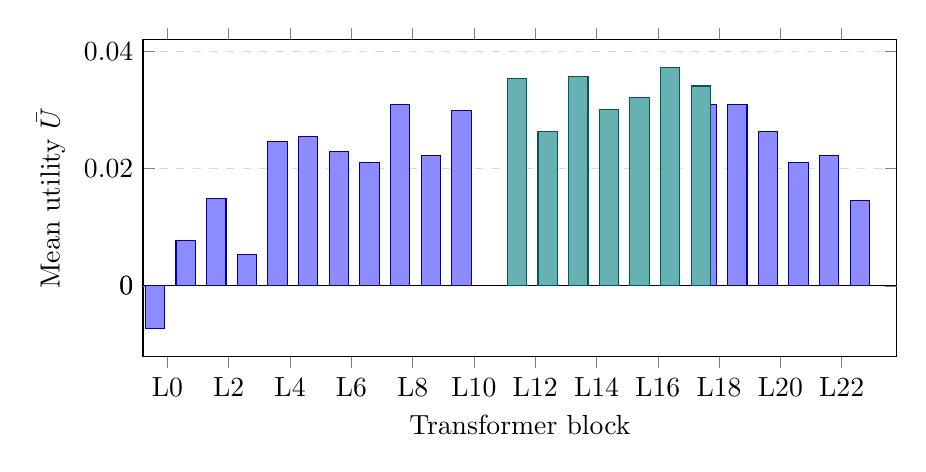
\begin{tikzpicture}
\begin{axis}[
    width=0.92\textwidth, height=5.6cm,
    ybar, bar width=7pt,
    xlabel={Transformer block}, ylabel={Mean utility $\bar U$},
    xtick={0,2,4,6,8,10,12,14,16,18,20,22},
    xticklabels={L0,L2,L4,L6,L8,L10,L12,L14,L16,L18,L20,L22},
    xmin=-0.8, xmax=23.8, ymin=-0.012, ymax=0.042,
    yticklabel style={/pgf/number format/fixed, /pgf/number format/precision=3},
    scaled y ticks=false,
    ymajorgrids=true, grid style={dashed, gray!30},
    extra y ticks={0}, extra y tick style={grid style={black, solid}},
]
\addplot[fill=blue!45, draw=blue!70!black] coordinates {
(0,-0.0073) (1,0.0077) (2,0.0149) (3,0.0053) (4,0.0246) (5,0.0255) (6,0.0230) (7,0.0210)
(8,0.0310) (9,0.0222) (10,0.0299) (18,0.0310) (19,0.0309) (20,0.0263) (21,0.0210) (22,0.0223) (23,0.0146)};
\addplot[fill=teal!60, draw=teal!70!black] coordinates {
(11,0.0354) (12,0.0263) (13,0.0357) (14,0.0301) (15,0.0322) (16,0.0372) (17,0.0341)};
\end{axis}
\end{tikzpicture}
\caption{Mean utility of each block over 3 seeds. The gain grows from L0, is highest in L11 to L17 (green) with a peak at L16 (+0.037), and drops again towards L23 (+0.015). Only L0 is below the decoder-only baseline.}
\label{fig:utility}
\end{figure*}

A few things are clear from these results. The block we adapt makes a real difference. Utility goes from $-0.007$ at L0 to $+0.037$ at L16, and every block except L0 beats the baseline. The highest mean utilities are at L16, L13, L11, L17 and L15, and the order of blocks is fairly similar across the three seeds (Kendall's $W = 0.73$).

The utility does not simply rise with depth. It rises, flattens out in the middle and then falls, like an upside-down U. A quadratic in depth explains $R^2 = 0.82$ of the variation, while a straight line explains only 0.26. L23, which is the top DSS block, comes 21st out of 24 by utility.

Single-block numbers are still uncertain. With three seeds, the median 95\% interval for one block is about $\pm 0.034$ wide, so we cannot reliably say which of two neighbouring blocks is better. The overall shape, low at the start, high in the middle and lower at the end, appears in all three seeds and also when tiles are resampled.

\section{Does DSS Predict the Gain?}

Table~\ref{tab:selectors} compares the DSS ranking and the simple rules with the measured utility order. R2 is the main DSS version used in Phase 2D and F is the Phase 2B-A ranking given above. The two give the same picture.

\begin{table}[t]
\centering
\caption{Rankings compared with measured utility. Regret is the utility lost against the best blocks, so lower is better. The Middle rule was chosen after seeing the results.}
\label{tab:selectors}
\small
\setlength{\tabcolsep}{3.5pt}
\begin{tabular}{@{}lcccc@{}}
\toprule
\textbf{Ranking} & \textbf{$\rho$} & \textbf{Partial} & \textbf{Top-1} & \textbf{Top-3} \\
\midrule
DSS (R2) & 0.420 & 0.076 & 0.015 & 0.029 \\
DSS (F) & 0.440 & 0.139 & 0.023 & 0.040 \\
MMD & $-0.077$ & 0.079 & 0.013 & 0.053 \\
Lowest-DSS & $-0.420$ & $-0.076$ & 0.045 & 0.086 \\
Early & $-0.422$ & 0 & 0.045 & 0.093 \\
Late & 0.422 & 0 & 0.023 & 0.050 \\
Middle & 0.632 & 0.728 & 0.002 & 0.017 \\
Random & 0.003 & n/a & 0.011 & 0.034 \\
\bottomrule
\end{tabular}
\end{table}

\begin{figure}[t]
\centering
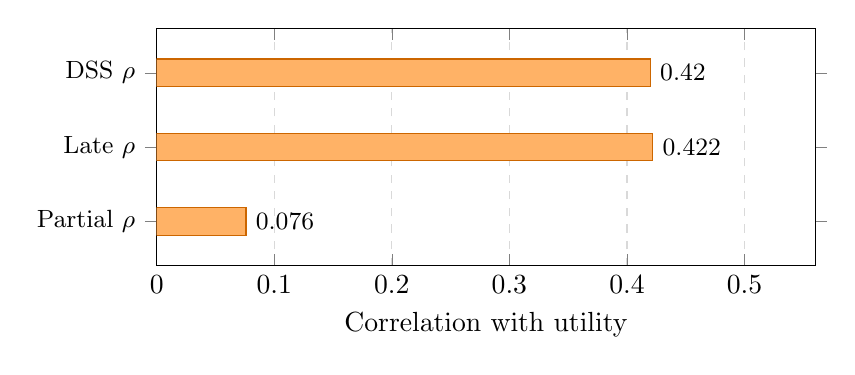
\begin{tikzpicture}
\begin{axis}[
    width=0.82\columnwidth, height=4.6cm,
    xbar, bar width=10pt,
    xlabel={Correlation with utility},
    ytick={0,1,2},
    yticklabels={{Partial $\rho$}, {Late $\rho$}, {DSS $\rho$}},
    y tick label style={font=\small},
    xmin=0, xmax=0.56,
    nodes near coords, nodes near coords style={font=\small, /pgf/number format/fixed, /pgf/number format/precision=3},
    xmajorgrids=true, grid style={dashed, gray!30},
    enlarge y limits=0.3,
]
\addplot[fill=orange!60, draw=orange!80!black] coordinates {(0.076,0) (0.422,1) (0.420,2)};
\end{axis}
\end{tikzpicture}
\caption{DSS correlates with utility about as much as the Late rule, and almost not at all once depth is removed.}
\label{fig:corr}
\end{figure}

\subsection{DSS is mostly depth}

The DSS order has a Spearman correlation of 0.420 with utility. The Late rule, which just ranks deeper blocks higher, gets 0.422. The gap between them is $-0.002$, with a tile-resampled 95\% interval of $-0.029$ to $+0.044$, so they are effectively the same (Figure~\ref{fig:corr}). After removing depth from both DSS and utility, the partial correlation is only 0.076. Whatever DSS says about utility, block depth already says it.

\subsection{Top-$k$ picks are no better than random}

Our failure test compares the DSS picks with random picks of the same size. Out of 20,000 random picks, the share that did at least as well as DSS was 0.67 for $k = 1$, 0.37 for $k = 3$ and 0.61 for $k = 5$. So DSS sits in the middle of the random results, and for $k = 1$ and $k = 5$ it is a little worse than the median random pick. The mean utility of the DSS top-$k$ blocks minus the mean of all 24 blocks is $-0.002$, $+0.003$ and $-0.001$ for $k = 1$, 3 and 5, which is no different from an average block.

\subsection{DSS picks the falling part of the curve}

Since DSS follows depth, it puts L19 to L23 at the top, and these are the blocks where utility is already going down. The top DSS block under R2 (L22) is 0.015 below the best block (L16), and L23 is 0.023 below L16. For L23 the 95\% interval of this difference does not include zero. This also explains the Phase 2C result. The DSS pair (L23, L19) did well with two blocks because deep blocks are fairly useful, not because DSS found the most useful ones.

\section{Phase 3: Reverse Transfer Setup}

Phase 3 reverses the transfer (Vaihingen to Potsdam). The Potsdam image and label archives matched their checksums, and all 38 label files were present. The split was frozen with 20, 8 and 10 tiles. The radiometric transform was refitted on the 20 Vaihingen training images. A colour check stopped the first data audit because a few pixels of label tile 4\_12 did not match the six class colours exactly. We approved a fixed rule that snaps a pixel to the nearest class colour only when the match is unambiguous, and recorded every snapped tile. The same rule was later needed for test tile 6\_7, where 0.7\% of pixels were snapped with a maximum colour distance of 3, against at least 249 to any other class.

\section{Phase 3: Single-Block Utility on Potsdam}

All 75 single-block runs on Potsdam passed the integrity checks: correct block and seed, unchanged backbone, matching initial states and data stream, exact checkpoint reload, and mIoU recomputed from the saved confusion matrices. The decoder-only validation mIoU was 0.5729, 0.5698 and 0.5646 for the three seeds (mean 0.569). Training took 24.3 hours in total, and the highest process peak was 10.31 GB. Figure~\ref{fig:utilityc} shows the mean utility of each block.

\begin{figure*}[t]
\centering
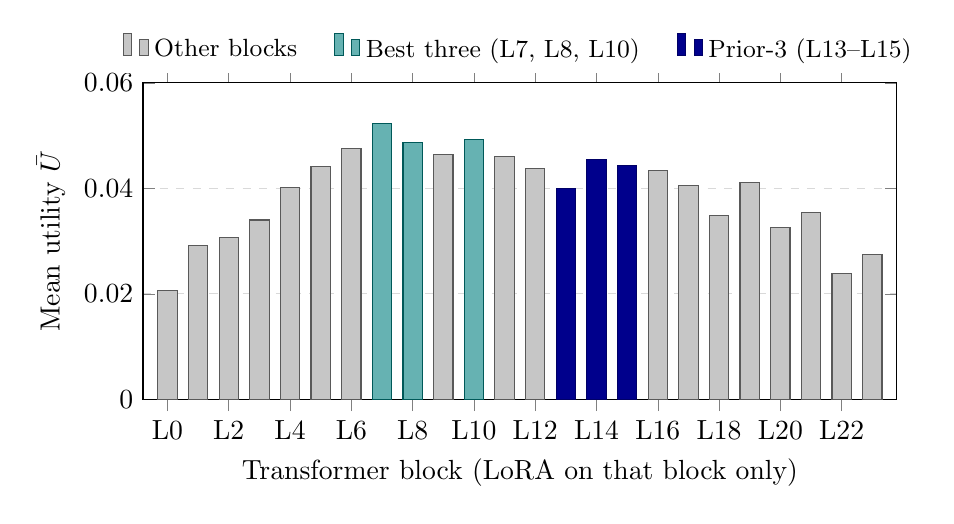
\begin{tikzpicture}
\begin{axis}[
    width=0.92\textwidth, height=5.6cm,
    ybar, bar width=7pt,
    xlabel={Transformer block (LoRA on that block only)}, ylabel={Mean utility $\bar U$},
    xtick={0,2,4,6,8,10,12,14,16,18,20,22},
    xticklabels={L0,L2,L4,L6,L8,L10,L12,L14,L16,L18,L20,L22},
    xmin=-0.8, xmax=23.8, ymin=0, ymax=0.06,
    yticklabel style={/pgf/number format/fixed, /pgf/number format/precision=3},
    scaled y ticks=false,
    ymajorgrids=true, grid style={dashed, gray!30},
    bar shift=0pt,
    legend style={at={(0.5,1.03)}, anchor=south, font=\small, draw=none, legend columns=3, /tikz/every even column/.append style={column sep=0.4cm}},
]
\addplot[fill=gray!45, draw=gray!70!black] coordinates {
(0,0.0206) (1,0.0292) (2,0.0306) (3,0.0340) (4,0.0402) (5,0.0442) (6,0.0476) (9,0.0464) (11,0.0460) (12,0.0438)
(16,0.0434) (17,0.0405) (18,0.0349) (19,0.0411) (20,0.0326) (21,0.0355) (22,0.0238) (23,0.0275)};
\addplot[fill=teal!60, draw=teal!70!black] coordinates {(7,0.0523) (8,0.0487) (10,0.0493)};
\addplot[fill=blue!55!black, draw=blue!40!black] coordinates {(13,0.0400) (14,0.0455) (15,0.0444)};
\legend{Other blocks, Best three (L7{,} L8{,} L10), Prior-3 (L13--L15)}
\end{axis}
\end{tikzpicture}
\caption{Mean utility of each block on Potsdam validation over 3 seeds, measured against the same-seed decoder-only run (mean 0.569). All 24 blocks help. The best block is L7 (+0.052) and the best three are L7, L10 and L8. The frozen depth prior's blocks (L13 to L15) are good but not the best.}
\label{fig:utilityc}
\end{figure*}

Three points stand out. First, every block helps, from +0.021 at L0 to +0.052 at L7, while on Vaihingen block L0 slightly hurt. Second, the curve still rises and then falls, but the peak moved earlier, from L16 on Vaihingen to L7 here. Third, the frozen depth prior still correlates with Potsdam utility ($\rho = 0.533$, Kendall 0.370), above the 0.3 threshold set in advance, so the prior counts as transferred. The Late rule, which prefers the deepest blocks, does not ($\rho = -0.125$). The mean seed standard deviation per block was 0.0043.

\section{Phase 3: Screening the Block Scores}

Table~\ref{tab:gate} shows each score against the measured utility and the four gate conditions.

\begin{table*}[t]
\centering
\caption{Screening of the block scores on Potsdam. $\rho$ is the Spearman correlation with $\bar U$, $r_{\text{res}}$ the residual correlation after the depth prior, LOSO the smallest leave-one-seed-out $r_{\text{res}}$, Boot the tile-bootstrap 2.5th percentile, and Regret the top-3 regret (the prior's is 0.0205). Fisher and LogME use labels and are references only.}
\label{tab:gate}
\small
\begin{tabular}{@{}llcccccc@{}}
\toprule
\textbf{Score} & \textbf{Top 3} & \textbf{$\rho$} & \textbf{$r_{\text{res}}$} & \textbf{LOSO} & \textbf{Boot} & \textbf{Regret} & \textbf{Gate} \\
\midrule
DSS-R2 & L4, L5, L3 & 0.476 & 0.446 & 0.367 & 0.384 & 0.0319 & fail (regret) \\
GSD sensitivity & L14, L13, L12 & 0.528 & $-0.057$ & $-0.078$ & $-0.106$ & 0.0210 & fail \\
IO-similarity & L0, L1, L2 & $-0.204$ & 0.583 & 0.570 & 0.554 & 0.0699 & fail (regret) \\
Activation norm & L23, L0, L22 & $-0.709$ & $-0.052$ & $-0.050$ & $-0.116$ & 0.0784 & fail \\
\midrule
Fisher (labels) & L12, L18, L21 & $-0.126$ & $-0.747$ & $-0.758$ & $-0.767$ & 0.0361 & reference \\
LogME (labels) & L7, L6, L8 & 0.496 & 0.336 & 0.260 & 0.220 & 0.0017 & reference \\
\midrule
Depth prior & L14, L13, L15 & 0.533 & -- & -- & -- & 0.0205 & transfers \\
\bottomrule
\end{tabular}
\end{table*}

No label-free score passed. DSS-R2 and input-output similarity carried information beyond the prior ($r_{\text{res}}$ of 0.446 and 0.583, stable across seeds and tiles), but their top three blocks were worse than the prior's, so they failed the regret condition. GSD sensitivity mostly copied the depth prior (its top three are almost the prior's), and activation norm was negatively related to utility. Among the label-using references, LogME found almost the best blocks (regret 0.0017), while Fisher's ranking was opposite to the residual utility.

DSS-R2 deserves a note. On Vaihingen its top blocks were the deepest ones, while on Potsdam its top blocks are L3 to L5, near the start of the network. A score that points to opposite ends of the network depending on the direction of transfer is not a stable guide for choosing blocks. By the rules written in advance, scenario S2 applied and C3 became the single confirmatory contrast.

\section{Phase 3: Budget-Matched Joint Adaptation}

All 67 joint-adaptation runs finished 2,000 steps and passed the same integrity checks as the single-block runs. Training took 24.1 hours in total and the highest process peak was 10.35 GB (uniform rank 1, seed 4000), under the 10.5 GB stop rule. Three runs were stopped by guards (the laptop sleeping on battery, swap growth while other apps were open, and a slow period over the runtime limit) and repeated under new IDs with the same seed and data. Table~\ref{tab:stagedval} gives the validation results.

\begin{table}[t]
\centering
\caption{Joint-adaptation validation mIoU (Potsdam, 8 tiles, step 2,000). Gain is over the K0 mean (0.5694).}
\label{tab:stagedval}
\small
\setlength{\tabcolsep}{4pt}
\begin{tabular}{@{}lccc@{}}
\toprule
\textbf{Arm} & \textbf{$n$} & \textbf{mIoU} & \textbf{Gain} \\
\midrule
Uniform rank 8 & 5 & 0.6810 & +0.112 \\
\textbf{Uniform rank 1} & 10 & \textbf{0.6647} & \textbf{+0.095} \\
Random-3 & 10 & 0.6392 & +0.070 \\
Fisher-3 & 5 & 0.6335 & +0.064 \\
LogME-3 & 5 & 0.6322 & +0.063 \\
Middle-3 & 5 & 0.6297 & +0.060 \\
Prior-3 & 10 & 0.6292 & +0.060 \\
DSS-R2-3 & 5 & 0.6267 & +0.057 \\
Late-3 & 5 & 0.6169 & +0.048 \\
K0 & 10 & 0.5694 & 0 \\
\bottomrule
\end{tabular}
\end{table}

At the matched budget, uniform rank 1 was clearly ahead of every 3-block arm. On validation, Prior-3 minus uniform rank 1 was $-0.0355$ on average with a standard deviation of only 0.0019, negative on all 10 seeds. The best 3-block arm was Random-3, ahead of every score-chosen set.

\section{Final Test on Potsdam}

After all 70 models (67 joint-adaptation models and the 3 reused single-block baselines) were integrity-checked, we froze a test manifest with every checkpoint hash, the 10 test tiles, and the hashes of the code and the analysis script. Each of the 700 tile evaluations ran in its own process, which could open only its own test tile. Every result file confirmed that only that tile's image and label were opened. One evaluation was stopped when a tile passed the 400-second per-tile limit during a temporary slowdown of the GPU (memory was normal). With approval, the run was resumed with a 900-second limit set in a separate launcher, so the hashed code was unchanged. The 97 finished tiles were kept, and the stopped tile was evaluated again from the start. Tile evaluations took about 130 to 145 seconds each, and the highest process peak was 6.0 GB.

\subsection{Confirmatory result}

Table~\ref{tab:c3} and Figure~\ref{fig:c3} give the C3 result.

\begin{table}[t]
\centering
\caption{Contrast C3 on the Potsdam test set (10 seeds, paired).}
\label{tab:c3}
\small
\begin{tabular}{@{}ll@{}}
\toprule
\textbf{Quantity} & \textbf{Value} \\
\midrule
Mean difference & $-0.0341$ \\
Standard deviation & 0.0070 \\
95\% $t$-interval & $[-0.0392,\ -0.0291]$ \\
Required lower bound & $> -0.010$ \\
Seeds with Prior-3 worse & 10 of 10 \\
Tile bootstrap 95\% & $[-0.0387,\ -0.0304]$ \\
Resamples above $-0.010$ & 0\% \\
\midrule
C3 (non-inferiority) & \textbf{not supported} \\
\bottomrule
\end{tabular}
\end{table}

\begin{figure}[t]
\centering
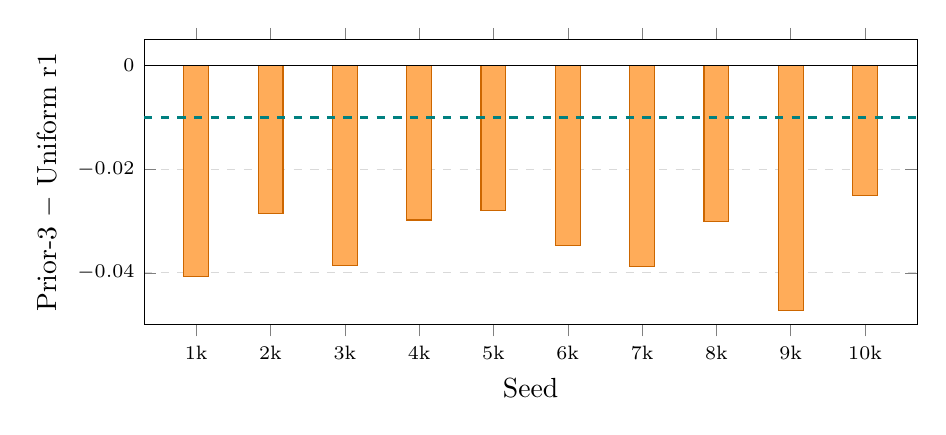
\begin{tikzpicture}
\begin{axis}[
    width=0.94\columnwidth, height=5.2cm,
    ybar, bar width=9pt,
    xlabel={Seed}, ylabel={Prior-3 $-$ Uniform r1},
    xtick={1,...,10}, xticklabels={1k,2k,3k,4k,5k,6k,7k,8k,9k,10k},
    x tick label style={font=\scriptsize},
    xmin=0.3, xmax=10.7, ymin=-0.05, ymax=0.005,
    yticklabel style={/pgf/number format/fixed, /pgf/number format/precision=2, font=\scriptsize},
    scaled y ticks=false,
    ymajorgrids=true, grid style={dashed, gray!30},
]
\addplot[fill=orange!65, draw=orange!80!black] coordinates {
(1,-0.0407) (2,-0.0285) (3,-0.0386) (4,-0.0298) (5,-0.0280) (6,-0.0348) (7,-0.0387) (8,-0.0300) (9,-0.0473) (10,-0.0250)};
\draw[teal, thick, dashed] (axis cs:0.3,-0.01) -- (axis cs:10.7,-0.01);
\draw[black] (axis cs:0.3,0) -- (axis cs:10.7,0);
\end{axis}
\end{tikzpicture}
\caption{Test-set difference between Prior-3 and uniform rank 1 for each seed. The dashed line is the non-inferiority margin ($-0.010$). Every seed is far below it.}
\label{fig:c3}
\end{figure}

The lower bound of the interval is about 0.029 below the margin, so non-inferiority is clearly rejected. The result does not depend on the choice of interval: the tile bootstrap gives almost the same range, and none of its 10,000 resamples came within the margin. The one-sided $p$-value for non-inferiority is essentially 1.

\subsection{All arms on the test set}

Table~\ref{tab:test} reports every arm on the test set. These numbers are descriptive.

\begin{table*}[t]
\centering
\caption{Potsdam test results (10 tiles) for all 70 models. mIoU is the mean over seeds with its 95\% interval, Gain is over the K0 mean (0.5285), and the class columns are mean IoU. Val is the validation mean from Table~\ref{tab:stagedval}.}
\label{tab:test}
\small
\setlength{\tabcolsep}{3pt}
\begin{tabular}{@{}lcccccccccc@{}}
\toprule
\textbf{Arm} & \textbf{$n$} & \textbf{Test mIoU} & \textbf{95\% interval} & \textbf{Gain} & \textbf{Val} & \textbf{Imp.} & \textbf{Bldg.} & \textbf{Low veg.} & \textbf{Tree} & \textbf{Car} \\
\midrule
Uniform rank 8 & 5 & 0.6270 & [0.6239, 0.6301] & +0.0985 & 0.6810 & 0.735 & 0.760 & 0.630 & 0.667 & 0.742 \\
\textbf{Uniform rank 1} & 10 & \textbf{0.6155} & [0.6106, 0.6203] & \textbf{+0.0869} & 0.6647 & 0.712 & 0.755 & 0.622 & 0.659 & 0.722 \\
Random-3 & 10 & 0.5904 & [0.5866, 0.5942] & +0.0619 & 0.6392 & 0.687 & 0.727 & 0.607 & 0.638 & 0.704 \\
Fisher-3 & 5 & 0.5835 & [0.5794, 0.5875] & +0.0549 & 0.6335 & 0.684 & 0.728 & 0.600 & 0.629 & 0.698 \\
LogME-3 & 5 & 0.5818 & [0.5769, 0.5866] & +0.0532 & 0.6322 & 0.676 & 0.709 & 0.605 & 0.636 & 0.695 \\
Middle-3 & 5 & 0.5816 & [0.5786, 0.5847] & +0.0531 & 0.6297 & 0.676 & 0.727 & 0.600 & 0.624 & 0.703 \\
Prior-3 & 10 & 0.5813 & [0.5786, 0.5841] & +0.0528 & 0.6292 & 0.681 & 0.708 & 0.601 & 0.623 & 0.699 \\
DSS-R2-3 & 5 & 0.5777 & [0.5714, 0.5840] & +0.0492 & 0.6267 & 0.670 & 0.689 & 0.608 & 0.635 & 0.695 \\
Late-3 & 5 & 0.5704 & [0.5657, 0.5750] & +0.0418 & 0.6169 & 0.664 & 0.710 & 0.593 & 0.611 & 0.673 \\
K0 & 10 & 0.5285 & [0.5245, 0.5325] & 0 & 0.5694 & 0.637 & 0.651 & 0.568 & 0.566 & 0.623 \\
\bottomrule
\end{tabular}
\end{table*}

\begin{figure}[t]
\centering
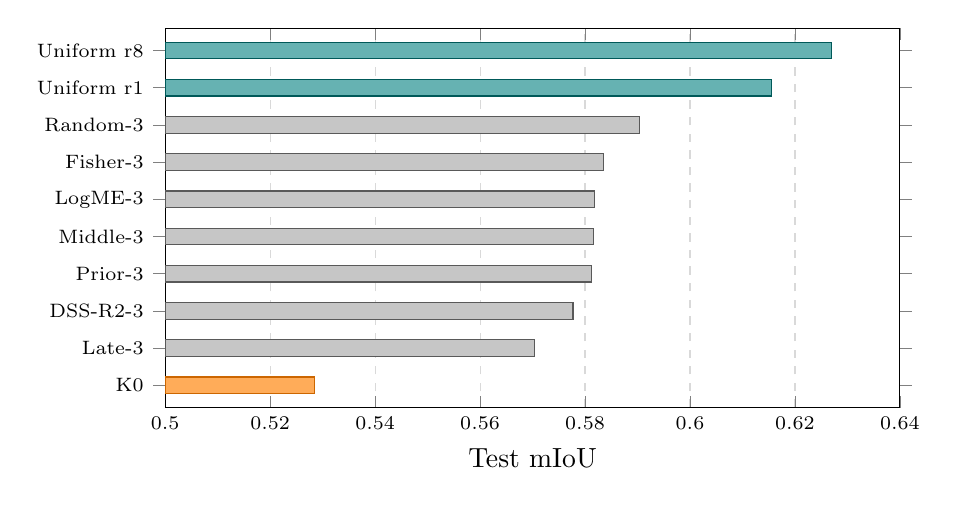
\begin{tikzpicture}
\begin{axis}[
    width=0.9\columnwidth, height=6.4cm,
    xbar, bar width=6pt,
    xlabel={Test mIoU},
    ytick={1,...,10},
    yticklabels={K0, Late-3, DSS-R2-3, Prior-3, Middle-3, LogME-3, Fisher-3, Random-3, Uniform r1, Uniform r8},
    y tick label style={font=\scriptsize},
    x tick label style={font=\scriptsize, /pgf/number format/fixed, /pgf/number format/precision=2},
    xmin=0.5, xmax=0.64, ymin=0.4, ymax=10.6,
    xmajorgrids=true, grid style={dashed, gray!30},
]
\addplot[fill=orange!65, draw=orange!80!black, bar shift=0pt] coordinates {(0.5285,1)};
\addplot[fill=gray!45, draw=gray!70!black, bar shift=0pt] coordinates {(0.5704,2) (0.5777,3) (0.5813,4) (0.5816,5) (0.5818,6) (0.5835,7) (0.5904,8)};
\addplot[fill=teal!60, draw=teal!70!black, bar shift=0pt] coordinates {(0.6155,9) (0.6270,10)};
\end{axis}
\end{tikzpicture}
\caption{Test mIoU of every arm. Uniform LoRA (green) beats every 3-block arm (grey) and the decoder-only baseline (orange).}
\label{fig:testarms}
\end{figure}

Four results stand out (Figure~\ref{fig:testarms}). First, adapting the backbone helps a lot on held-out tiles: every arm gains between +0.042 and +0.099 over the decoder-only baseline, and the intervals across seeds are narrow. Second, uniform rank 1 keeps 88\% of the gain of uniform rank 8 ($0.0869 / 0.0985$) with one eighth of its LoRA parameters. Third, no block-scoring method beat random selection: Random-3 was the best 3-block arm, and paired by seed with uniform rank 1, the 3-block arms were behind by 0.025 (Random-3) to 0.043 (Late-3). Fourth, the arm ranking on the test set is exactly the same as on validation, and every arm loses a similar 0.04 to 0.05 from validation to test, which suggests that the validation tiles were not overfitted. The car class gains the most from adaptation, and clutter (not shown, IoU 0.13 to 0.23) stays the hardest class for every arm.


% =======================================================
% ============ CHAPTER 6: DISCUSSION & LIMITATIONS ======
% =======================================================
\chapter{Discussion and Limitations}
\label{ch:discussion}

\section{What the Results Mean}

The project started from a simple idea: if the domain shift mostly affects some blocks of a frozen model, adapting only those blocks should be enough. The experiments support the first half of this idea and reject the second.

Which block is adapted does matter. In both directions, single-block LoRA gave clearly different gains at different depths, with an upside-down U shape. But the location of the best blocks changed with the direction of transfer (L11 to L17 for Vaihingen, L7 to L10 for Potsdam), and none of our scores followed this change. DSS measures a real feature difference, but its normalisation is dominated by how little natural spread the deep blocks have, so it ends up as a stand-in for depth. In the reverse direction it even pointed to the earliest blocks. The other label-free scores either copied the depth prior or pointed to the wrong blocks, and the label-using scores were no better than random once three blocks were trained together.

The budget-matched comparison gives the clearest message. Every block helps on its own, so a method that leaves 21 of 24 blocks untouched gives up gains that a rank-1 update can collect almost for free. With exactly the same 98,304 LoRA parameters, spreading them as rank 1 over all blocks beat every way of choosing three blocks at rank 8, by 2.5 to 4.3 mIoU points on the test set. Uniform rank 1 also kept 88\% of the gain of standard rank-8 LoRA with one eighth of its LoRA parameters.

\begin{table}[t]
\centering
\caption{Summary of the final evidence.}
\label{tab:summary}
\small
\begin{tabular}{@{}p{3.6cm}p{3.6cm}@{}}
\toprule
\textbf{Supported} & \textbf{Not supported} \\
\midrule
LoRA gives large, stable gains (+0.042 to +0.099 test mIoU) & DSS finds the useful blocks \\
Blocks differ in utility, with an upside-down U over depth & Any label-free score passing the screening gate \\
Uniform rank 1 keeps 88\% of rank-8 gain with 1/8 of the LoRA parameters & 3 chosen blocks matching uniform rank 1 at equal budget \\
Same ranking of methods on validation and test & Chosen blocks beating random blocks \\
\bottomrule
\end{tabular}
\end{table}

\section{Why We Trust the Results}

Table~\ref{tab:summary} summarises the evidence. We trust it for five reasons. Every split, score, threshold, set of arms and analysis script was frozen and hashed before the data that would judge it existed. The final claim rests on a single confirmatory test, so there is no multiple-testing problem. All comparisons are paired by seed, with identical starting weights and data order checked by hash. The main effect is large compared with the noise: the difference between the 3-block prior and uniform rank 1 is about five standard deviations of the paired difference, with the same sign on every seed and almost every tile resample. Finally, the test tiles were opened only once, for frozen models, and every test result records which files were opened. The ranking of all ten methods was the same on the validation and the test tiles.

\section{Limitations}

All results come from one backbone (Prithvi-EO-2.0-300M) and one pair of cities (ISPRS Potsdam and Vaihingen), with LoRA on the query and value projections only, a decoder that reads only the last block, and 2,000 training steps. A different backbone, decoder, training length or type of shift may change the picture.

Uniform LoRA was tested only at ranks 1 and 8, so we do not know the best rank for a given budget. Full fine-tuning could not be run within the 16 GB memory of our laptop, so we cannot compare against it.

The secondary methods used 5 seeds and the random arm used one seed per random draw, so their small differences are not reliable. Only the comparison of the depth prior with uniform rank 1 is confirmatory.

The test tiles come from one city, so the tile bootstrap measures variation within Potsdam, not across cities. The Vaihingen test tiles were kept locked throughout and have not been used.

% =======================================================
% ============ CHAPTER 7: CONCLUSION ====================
% =======================================================
\chapter{Conclusion and Future Work}
\label{ch:conclusion}

\section{Conclusion}

In this project we designed, implemented and tested DSSA, a way of choosing which blocks of a geospatial foundation model to adapt with LoRA under domain shift, and we compared it with simply spreading LoRA over all blocks. Our final findings are as follows.

Adapting the model is clearly worthwhile. Every adaptation method improved on the decoder-only model, by +0.042 to +0.099 mIoU on the held-out Potsdam test tiles, and the results were stable across seeds.

Which block is adapted matters, but our scores cannot tell which. DSS is mostly a depth ranking, it did not beat random picks, and it pointed to opposite ends of the network in the two directions. Five further scores did not help either.

Selecting blocks lost to spreading the budget. At an equal budget of 98,304 LoRA parameters, the best frozen choice of three blocks scored 0.034 mIoU below uniform rank-1 LoRA on the test set (95\% interval $-0.039$ to $-0.029$), worse on all 10 seeds, and no choice of three blocks beat three random blocks. Uniform rank-1 LoRA reached 0.615 test mIoU and kept 88\% of the gain of standard rank-8 LoRA with one eighth of its LoRA parameters.

In short: \textit{spread, don't select}. For adapting Prithvi-EO-2.0 to a new aerial domain under a tight parameter budget, a very small rank on every block is a simple, strong and cheap choice.

\section{Future Work}

First, the study should be repeated on a different dataset and type of shift, for example the Urban and Rural domains of LoveDA \cite{wang2021loveda}, before the conclusion is generalised. Second, a rank sweep for uniform LoRA (ranks 1, 2, 4 and 8) would show the best use of a given budget. Third, the locked Vaihingen test tiles can be used once to check the first single-block study on held-out data. Fourth, comparisons with full fine-tuning and with other backbones would need a machine with more memory. Finally, we plan to write up the study as a 4-page IEEE paper for IGARSS 2027, with the working title ``Spread, Don't Select: Budget-Matched LoRA Placement for Cross-Domain Segmentation with Prithvi-EO-2.0''.

% =======================================================
% ==================== REFERENCES =======================
% =======================================================
\small
\setstretch{1.0}
\bibliographystyle{plainnat}
\begin{thebibliography}{50}
\setlength{\itemsep}{1pt}

\bibitem[Ben-David et~al.(2010)]{bendavid2010theory}
Ben-David, S., Blitzer, J., Crammer, K., Kulesza, A., Pereira, F., and Vaughan, J.~W. (2010).
A theory of learning from different domains.
\emph{Machine Learning}, 79(1--2):151--175.

\bibitem[Cong et~al.(2022)]{cong2022satmae}
Cong, Y., Khanna, S., Meng, C., Liu, P., Rozi, E., He, Y., Burke, M., Lobell, D.~B., and Ermon, S. (2022).
SatMAE: Pre-training transformers for temporal and multi-spectral satellite imagery.
In \emph{NeurIPS}.

\bibitem[Dosovitskiy et~al.(2021)]{dosovitskiy2021image}
Dosovitskiy, A., Beyer, L., Kolesnikov, A., et~al. (2021).
An image is worth 16x16 words: Transformers for image recognition at scale.
In \emph{ICLR}.

\bibitem[Ganin et~al.(2016)]{ganin2016domain}
Ganin, Y., Ustinova, E., Ajakan, H., Germain, P., Larochelle, H., Laviolette, F., Marchand, M., and Lempitsky, V. (2016).
Domain-adversarial training of neural networks.
\emph{Journal of Machine Learning Research}, 17(59):1--35.

\bibitem[Gretton et~al.(2012)]{gretton2012kernel}
Gretton, A., Borgwardt, K.~M., Rasch, M.~J., Sch{\"o}lkopf, B., and Smola, A. (2012).
A kernel two-sample test.
\emph{Journal of Machine Learning Research}, 13:723--773.

\bibitem[He et~al.(2022)]{he2022masked}
He, K., Chen, X., Xie, S., Li, Y., Doll{\'a}r, P., and Girshick, R. (2022).
Masked autoencoders are scalable vision learners.
In \emph{Proceedings of the IEEE/CVF CVPR}, pages 16000--16009.

\bibitem[Houlsby et~al.(2019)]{houlsby2019parameter}
Houlsby, N., Giurgiu, A., Jastrzebski, S., Morrone, B., de~Laroussilhe, Q., Gesmundo, A., Attariyan, M., and Gelly, S. (2019).
Parameter-efficient transfer learning for NLP.
In \emph{ICML}, pages 2790--2799.

\bibitem[Hu et~al.(2022)]{hu2022lora}
Hu, E.~J., Shen, Y., Wallis, P., Allen-Zhu, Z., Li, Y., Wang, S., Wang, L., and Chen, W. (2022).
LoRA: Low-rank adaptation of large language models.
In \emph{ICLR}.

\bibitem[Jakubik et~al.(2023)]{jakubik2023foundation}
Jakubik, J., Roy, S., Phillips, C.~E., et~al. (2023).
Foundation models for generalist geospatial artificial intelligence.
\emph{arXiv preprint arXiv:2310.18660}.

\bibitem[Kirkpatrick et~al.(2017)]{kirkpatrick2017overcoming}
Kirkpatrick, J., Pascanu, R., Rabinowitz, N., et~al. (2017).
Overcoming catastrophic forgetting in neural networks.
\emph{Proceedings of the National Academy of Sciences}, 114(13):3521--3526.

\bibitem[Kornblith et~al.(2019)]{kornblith2019similarity}
Kornblith, S., Norouzi, M., Lee, H., and Hinton, G. (2019).
Similarity of neural network representations revisited.
In \emph{ICML}, pages 3519--3529.

\bibitem[Lee et~al.(2023)]{lee2023surgical}
Lee, Y., Chen, A.~S., Tajwar, F., Kumar, A., Yao, H., Liang, P., and Finn, C. (2023).
Surgical fine-tuning improves adaptation to distribution shifts.
In \emph{ICLR}.

\bibitem[Long et~al.(2015)]{long2015fully}
Long, J., Shelhamer, E., and Darrell, T. (2015).
Fully convolutional networks for semantic segmentation.
In \emph{Proceedings of the IEEE CVPR}, pages 3431--3440.

\bibitem[Loshchilov and Hutter(2019)]{loshchilov2019decoupled}
Loshchilov, I. and Hutter, F. (2019).
Decoupled weight decay regularization.
In \emph{ICLR}.

\bibitem[Milletari et~al.(2016)]{milletari2016vnet}
Milletari, F., Navab, N., and Ahmadi, S.-A. (2016).
V-Net: Fully convolutional neural networks for volumetric medical image segmentation.
In \emph{International Conference on 3D Vision (3DV)}, pages 565--571.

\bibitem[Raghu et~al.(2017)]{raghu2017svcca}
Raghu, M., Gilmer, J., Yosinski, J., and Sohl-Dickstein, J. (2017).
SVCCA: Singular vector canonical correlation analysis for deep learning dynamics and interpretability.
In \emph{NeurIPS}.

\bibitem[Rottensteiner et~al.(2012)]{rottensteiner2012isprs}
Rottensteiner, F., Sohn, G., Jung, J., Gerke, M., Baillard, C., Benitez, S., and Breitkopf, U. (2012).
The ISPRS benchmark on urban object classification and 3D building reconstruction.
\emph{ISPRS Annals of the Photogrammetry, Remote Sensing and Spatial Information Sciences}, I-3:293--298.

\bibitem[Szwarcman et~al.(2024)]{szwarcman2024prithvi}
Szwarcman, D., Roy, S., Fraccaro, P., et~al. (2024).
Prithvi-EO-2.0: A versatile multi-temporal foundation model for Earth observation applications.
\emph{arXiv preprint arXiv:2412.02732}.

\bibitem[Tuia et~al.(2016)]{tuia2016domain}
Tuia, D., Persello, C., and Bruzzone, L. (2016).
Domain adaptation for the classification of remote sensing data: An overview of recent advances.
\emph{IEEE Geoscience and Remote Sensing Magazine}, 4(2):41--57.

\bibitem[Wang et~al.(2021)]{wang2021loveda}
Wang, J., Zheng, Z., Ma, A., Lu, X., and Zhong, Y. (2021).
LoveDA: A remote sensing land-cover dataset for domain adaptive semantic segmentation.
In \emph{NeurIPS Datasets and Benchmarks Track}.

\bibitem[Yosinski et~al.(2014)]{yosinski2014transferable}
Yosinski, J., Clune, J., Bengio, Y., and Lipson, H. (2014).
How transferable are features in deep neural networks?
In \emph{NeurIPS}, pages 3320--3328.

\bibitem[You et~al.(2021)]{you2021logme}
You, K., Liu, Y., Wang, J., and Long, M. (2021).
LogME: Practical assessment of pre-trained models for transfer learning.
In \emph{ICML}, pages 12133--12143.

\bibitem[Zhang et~al.(2023)]{zhang2023adalora}
Zhang, Q., Chen, M., Bukharin, A., He, P., Cheng, Y., Chen, W., and Zhao, T. (2023).
Adaptive budget allocation for parameter-efficient fine-tuning.
In \emph{ICLR}.

\end{thebibliography}

\end{document}
